\begin{abstract}

The O-Crab is an autonomous biologically inspired robot designed to navigate the harsh conditions and terrain of waterfronts and collect the ever increasing amounts of litter found near waterways. To do so, it is equipped with five crab-like legs, each providing two degrees of freedom. These legs are powered by a set of motors and harmonic drive reducers. The O-Crab's fully waterproof construction and resistant materials enable it to operate in moisture and potentially salt intensive environments. Thanks to lid-mounted solar panels, it operates independently from centralized electricity sources and for long periods of time by alternating between solar power and the on-board batteries.

\begin{figure}[H]
    \centering
    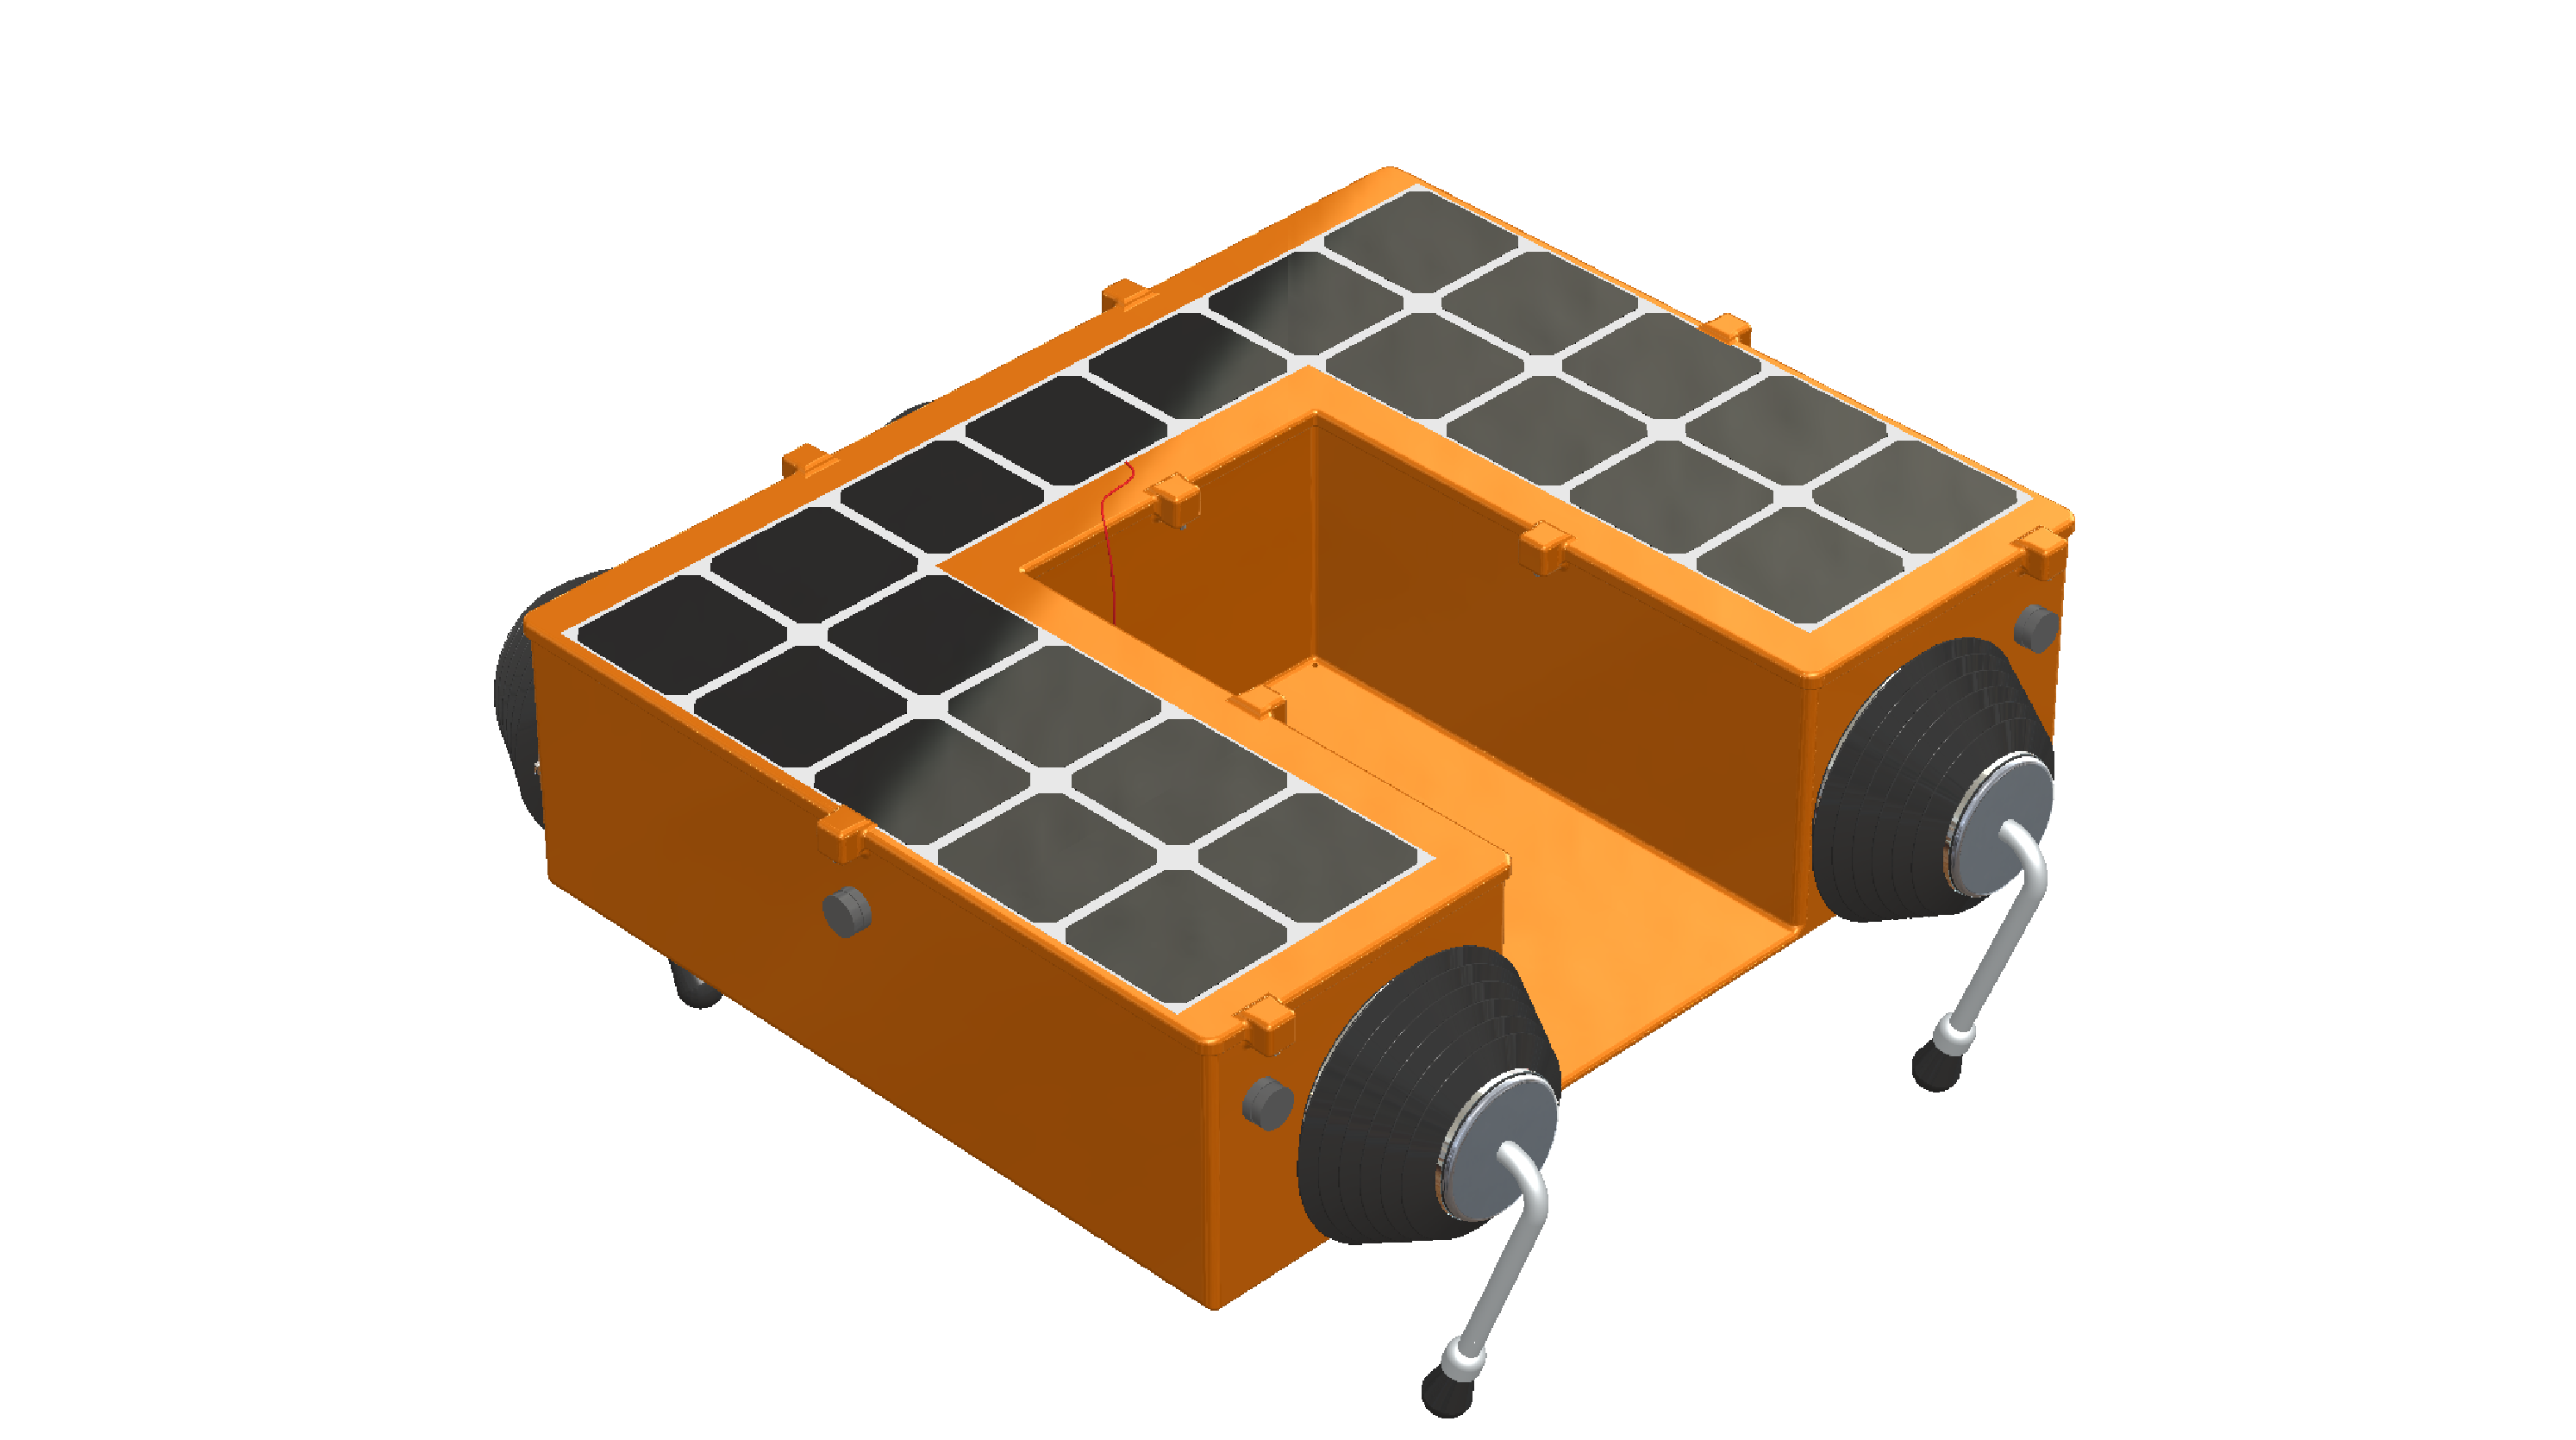
\includegraphics[width=\textwidth]{01_Abstract/img/IsoView.PNG}
    \caption{The O-Crab waterfront robot}
    \label{fig:abstract}
\end{figure}
    
    
\end{abstract}